\chapter{Descripción del sistema de software}\label{sistema_de_software}

\section{Introducción}

En el capítulo~\ref{chap:algoritmos} se ha hecho una revisión de los algoritmos que hacen separación de una silueta de su imagen de fondo (\textit{Background Subtraction}), específicamente en algoritmos basados en mixtura de componentes gaussianos (\textit{Gaussian Mixture Model}). Posteriormente, en el capítulo~\ref{chap:metricas} se hizo una descripción de las principales métricas utilizadas en la comunidad de investigación de visión por computador, para hacer evaluación de rendimiento de estos algoritmos. El siguiente paso, es colocar ambos elementos en el contexto de este trabajo, en una herramienta de software disponible para la comunidad de investigación, que permita incluir nuevos desarrollos y sea de utilidad para hacer evaluación de algoritmos. Se requiere entonces articular ambas áreas en una herramienta de software que permita utilizar uno de estos algoritmos sobre el conjunto de datos MuHAVI, y emplear las métricas de rendimiento para  obtener una idea global de desempeño del algoritmo seleccionado. Este capítulo se enfoca en el proceso de desarrollo de software que finaliza con la implementación de ambos elementos (algoritmos y métricas de desempeño) en dos módulos que constituyen el producto final de software, y cumple con los requerimientos planteados en el capítulo~\ref{chap:capitulo_1}. Se hace una descripción de los distintas etapas metodológicas involucradas en el desarrollo del sistema de software, se discute el diseño y la estructura de software propuesto, así como las principales herramientas (\textit{OpenCV}) escogidas para realizar el desarrollo.

% los requerimientos definidos se establecen dos escenarios de casos de usos
%
%(obtenidas previamente) Una segunda parte se publicar las siluetas generadas.  utilizar el conjunto de daten un comienzo se plantea uti
%
%Este proyecto en un comienzo se plantea varios desafíos; utilizar MuHAVI como conjunto de datos de experimentación al ser una base de datos usadas por más de 150 personas en el mundo, se planteaba que era un conjunto de datos tui aprovechar las características de MuHAVI\cite{singh_muhavi_2010} como conjunto de datos de experimentación,  
%- en esta base de datos tambien seria bueno aplicar un buen metodo de separacion de foreground para aumentar sustancialmente el numero de ejemplos de acciones.
%
%Se me ocurre mas o menos esto
%\begin{itemize}
%\item Centrarse en MuHAVI http://dipersec.king.ac.uk/MuHAVi-MAS/, es una base de datos usadas por mas de 150 personas en el mundo
%\item Adaptar el metodo de foreground detection de Z Chen y procesar todo el MuHavi (yo tengo los videos originales completos) para generar "state-of-the-art" siluetas
%\item Publicar las siluetas (para que la gente las use)
%\item Comparar las siluetas con las manuales y publicar un paper comparando este metodo con otros metodos de foreground detection
%\item Implementar un metodo de deteccion de actividad (por ejemplo el de Zaragoza mas otro que sea state of the art) y hacer un estudio comparativo usando MuHAvi
%\item Publicar los resultados de ( 5)
%Con eso creo que es suficiente.
%\end{itemize}
%
%Me gustaria que hicieramos todo el codigo en OpenCV con Linux (you uso Linux Mint que es derivado de Ubuntu, Ubuntu tambien me gusta)



\newpage
\section{Captura de requerimientos}

Se plantea en el comienzo del proyecto la idea de aprovechar las características de MuHAVI \cite{singh_muhavi_2010} como conjunto de datos de experimentación, para ser utilizada con el método de \textit{Foreground Detection} propuesto por Zezhi Chen\cite{chen_vehicle_2012}, un algoritmo orientado a  realizar seguimiento y detección de vehículos, el cual podría ser aplicado para generar  y colocar a disposición de la comunidad de investigación, todas las siluetas generadas a partir este método. En una segunda instancia se propone comparar las siluetas manuales (\textit{ground-truth}) que tiene MuHAVI con los resultados de este método y otros métodos adicionales similares. Una última parte implementar algún método de detección de actividad y hacer un estudio comparativo.

%(con la finalidad de colocar) 

De este plan inicial y después de varias revisiones, surgen los objetivos del proyecto registrados en el capítulo~\ref{chap:capitulo_1}, y que sirven de base de los requerimientos funcionales capturados para el desarrollo de la implementación de esta herramienta, que se describen a continuación.

\begin{itemize}
\item Desarrollar un software como sistema base, para incorporar algoritmos que utilicen métodos de separación de siluetas de su imagen de fondo (\textit{Foreground Detection} o \textit{Background Subtraction})
\item Implementar el algoritmo \textit{SAGMM}\cite{chen_vehicle_2012} (\textit{Self-Adaptive Gaussian Mixture Model}) de separación de la siluetas de su imagen del fondo e incorporarlo en el sistema base. 
\item Implementar una herramienta de software que consolide las métricas escogidas para realizar una evaluación global de desempeño del resultado de estos algoritmos.
\end{itemize}

Con los requerimientos definidos se establecen dos escenarios de casos de usos, realizado por dos actores: un investigador que ejecuta y verifica los algoritmos, y la comunidad de investigación (otro actor  investigador) que utiliza la herramienta con las métricas y evalúa resultados. Ambos casos de uso se ilustran en la figura~\ref{fig:ch5:use_case}. En este primer prototipo se dejan fuera varios escenarios, como los casos de fallas y el procedimiento de compilar el programa ejecutable para agregar un nuevo algoritmo en el sistema principal.


\begin{itemize}
\item \textbf{Caso de uso 1}: Ejecutar algoritmo para verificación.\\
Investigador agrega nuevo algoritmo desarrollado en la comunidad en el sistema de software para utilizarlo y verificarlos con el conjunto de datos MuHAVI.
\begin{enumerate}
\item Investigador modifica archivos de configuración para incluir algoritmo en el sistema
\item Investigador ejecuta programa principal con base datos MuHAVI 
\item Investigador verifica siluetas obtenidas después del procesamiento
\end{enumerate}

\item \textbf{Caso de uso2}: Obtener desempeño general de algoritmo
\begin{enumerate}
\item Investigador obtiene siluetas resultantes de un procesamiento anterior.
\item Investigador obtiene imágenes de referencia \textit{ground-truth} provenientes de MuHAVI.
\item Investigador ejecuta herramientas de medición de desempeño.
\end{enumerate}
\end{itemize}



\begin{figure}[h!]
\centering
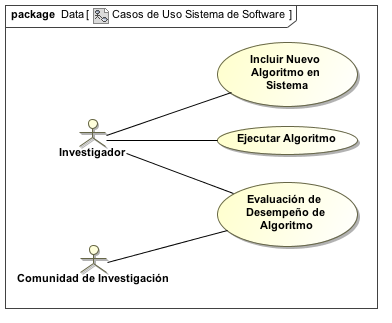
\includegraphics[scale=1.0]{img/ch5/use_case}
\caption[Casos de uso de los requerimientos establecidos en el proyecto]{Casos de uso de los requerimientos establecidos en el proyecto. El investigador agrega y utiliza un algoritmo desde el sistema. El investigador usa la herramienta de métricas para obtener evaluación de desempeño y los coloca a disposición de la comunidad (la comunidad de investigación usa los resultados obtenidos).}
\label{fig:ch5:use_case}
\end{figure}



%\section{Decisiones de diseño}
%
%La solución de software implementada, es un conjunto de bibliotecas desarrolladas en lenguaje de programación C++ orientado a objetos. Estas consisten, en un grupo de clases que posibilitan por una parte, construir una aplicación cliente para incorporar los algoritmos de visión de computador que se intentan verificar, y por otra parte, evaluar resultados logrados con este cliente (u otra aplicación similar). 
%Comparando el resultado obtenido con imágenes de referencias, suministradas por el conjunto de datos de evaluación. El software proporciona las interfaces necesarias, que simplifican la creación de instancias de los distintos algoritmos, incluidos en el sistema de software. Facilita también, la incorporación de nuevos algoritmos, encapsulando las bibliotecas (de estos algoritmos) en una clase que contiene las operaciones predeterminadas, reconocidas por el sistema de software. 
%
%Otro aspecto importante de esta solución de software, constituye la herramienta de evaluación de desempeño. Ésta fue proyectada, desde un principio, como un cliente que recibe de entrada un conjunto de imágenes procesadas, y otro conjunto de imágenes de referencia (\textit{ground-truth}). El resultado es un resumen de desempeño, producto de la comparación de cada imagen de ambos conjuntos. Este diseño, es independiente de la plataforma sobre el cual se ejecuta el algoritmo medido. La evaluación se realiza sobre imágenes resultantes, las cuales fueron previamente procesadas por los algoritmos que se intentan valorar. Esta herramienta de software, incluye las métricas más comunes utilizadas en segmentación de imágenes, y un par de métricas relacionadas con la medición de percepción: similaridad estructural \cite{park_benchmark_2013, wang_image_2004}, y D-Score\cite{lallier_testing_2011}. El producto final es un archivo de texto, que contiene los resultados obtenidos para cada imagen y un valor acumulado total que informa el desempeño global del algoritmo logrado en toda la secuencia.

\section{Arquitectura de sistema de software}

El diseño de la arquitectura de software está basada en módulos independientes constituida en una estructura de tres capas; herramientas base, núcleo del software, y herramientas de software. Cada módulo dentro de una capa, es una unidad funcional independiente, que suministra bibliotecas de clases para construir los programas o clases de los módulos en las capa superiores. Asimismo, los módulos de un mismo nivel pueden utilizar las bibliotecas de sus vecinos, como el caso, de los programas utilitarios ubicados en la capa del medio. La imagen de la figura \ref{fig:arq_software} es una vista a nivel de módulos, de la arquitectura de software diseñada para esta solución, una descripción más detallada por módulo se realiza en la siguiente sección. Los módulos de la parte inferior de esta imagen (en color naranja pálido) corresponden a todas las biblioteca de software externas, utilizadas para construir este software. Los módulos localizados en la parte media y superior, son los distintos componentes implementados en este proyecto. 

El diseño del software en módulos se basa principalmente en la independencia de los requerimientos. Cada módulo es una unidad de implementación independiente que se relaciona con los requisitos establecidos. El sistema base para incluir algoritmos y la herramienta de métricas, son unidades que están definidas para funcionar independiente y no esta dentro de los requerimientos que funcionen en forma simultánea. Esta estructura además permite mejorar tareas de mantenimiento, depuración y arreglo de problemas, porque permite enfocarse directamente en el módulo que requiere mejorarse y no perturba el funcionamiento del otro módulo.
 
Descripción de los módulos señalados en el diagrama en la figura \ref{fig:arq_software}.
\begin{itemize}
  \item \textbf{Herramientas de desarrollo:} es el módulo que proporciona compiladores, programas de configuración para construir la solución de software.
  \item \textbf{OpenCV:} es un conjunto de bibliotecas C++ de software abierto (\textit{Open Source}) usadas en vision por computador.
  \item \textbf{Biblioteca Boost:} Utilizada para el manejo de caracteres y \textit{strings} en C++, expresiones regulares y control de opciones de entrada en programa principal.
  \item \textbf{Sistema Base:} Parte principal del software, éste realiza integración de algoritmos de separación \textit{foreground} y \textit{backgorund}.
  \item \textbf{Medición de desempeño:} Esta parte incorpora todas las métricas que posibilitan hacer evaluación de performance.
  \item \textbf{Programas Utilitarios:} Conjunto de clases y programas básicos que sirven de apoyo a los otros módulos.   
  \item \textbf{Algoritmos}: Esta módulo proporciona las clases que encapsulan los diferentes algoritmos, que se intenta evaluar.
  \item \textbf{Scripts de Análisis:} Programas desarrollados en lenguaje de programación \textit{Python} que ayudan en la creación de gráficas de desempeños, empleados para hacer análisis de los datos resultantes.
  \item \textbf{Aplicaciones:} Esta parte corresponde a los clientes que hacen uso de las herramientas proporcionadas por este sistema de software. 
\end{itemize}

\begin{figure}[h!]
\centering
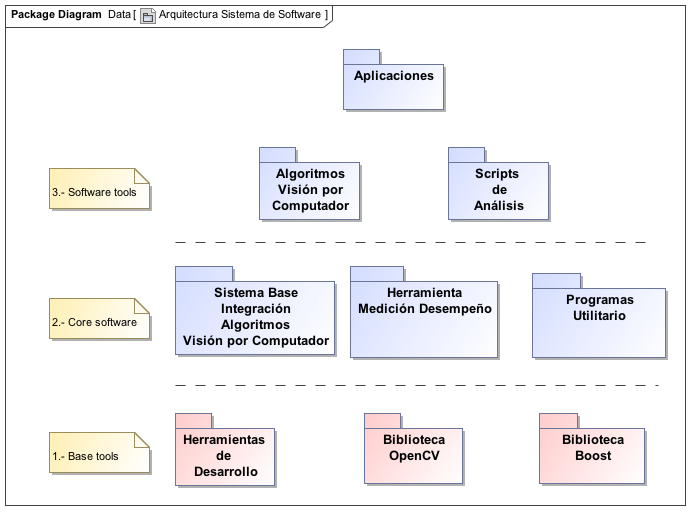
\includegraphics[scale=0.7]{img/ch5/BGS_Architecture}
\caption[Arquitectura modular de software]{Diagrama de la arquitectura de software. Se definen tres niveles de capas, la capa inferior suministras las herramientas base (clases, bibliotecas, archivos de configuración) para construir las capas superiores. La capa del medio comprende distintos módulos que constituyen el núcleo del sistema de software, en esta capa se coloca la implementación de la herramienta de métricas, el sistema base que incorpora los algoritmos que se intenta evaluar, y programas utilitarios. La última capa contiene los módulos con las bibliotecas de los algoritmos y programas de \textit{scripting} que ayudan en el análisis de las métricas de rendimiento.}
\label{fig:arq_software}
\end{figure}

\section{Herramientas de Soporte Base}

\subsection{Herramientas de desarrollo}
El desarrollo de los diferentes módulos de software ha sido realizado en una distribución Linux, \textbf{\textit{Ubuntu} 12.04 LTS precise}. Ubuntu es un sistema operativo Linux, basado en Debian, que incluye todas las herramientas necesarias, para hacer la implementación de los paquetes de software de esta solución. Abajo se especifican las principales herramientas involucradas en el de desarrollo.

\begin{itemize}
\item \textbf{Compilador:} GNU GCC versión 4.6
\item \textbf{CMake:} Grupo de herramientas, \textit{Open Source} independiente del sistema operativo, diseñado para construir, validar paquetes de software. Se ha usado esencialmente para generar los archivos \textit{Makefile} nativos al sistema operativo Ubuntu. La utilidad de CMake, radica en la independencia de la plataforma sobre la cual se está desarrollando. De esta manera, en caso de ser necesario, los módulos de software también pueden ser compilados y ejecutados en otros ambientes (\textit{MAC OS X}, otros ``distros'' de \textit{Linux}, o \textit{Windows}).
\item \textbf{Servidor de repositorios \textit{GitHub}}\cite{github}\textit{:} Mantiene control de cambios de versión de los distintos módulos. Este servicio de repositorios público, se basa en \textit{GIT} un sistema de control de versiones distribuidos. Las principales características, entre otras, es un sistema de control de los datos, almacena el estado de un proyecto a nivel de directorios y archivos. Crea un registro completo (\textit{snapshot}) del repositorio que esta siendo almacenado, esto facilita las tareas de recuperación, creación de ramas de desarrollo (\textit{branch}) y unión (\textit{merge}) de diferentes versiones de un módulo. El proyecto completo puede ser localizado en el siguiente URL:\textit{ \textit{https://github.com/jorgesep/BGS}}. 
\end{itemize}

\subsection{Biblioteca OpenCV de Visión por Computador}
OpenCV\cite{opencv} (\textit{Open Source Computer Vision Library}) es una biblioteca especializada en visión por computador, facilita una API (\textit{Application Programming Interface}) con una serie de módulos necesarios para construir una aplicación en visión por computador. El módulo principal, define las estructuras básicas, sobre la cual se desarrollan muchas de las aplicaciones, incluido los módulos de software construidos en este proyecto de tesis. OpenCV define, un grupo de tipos básicos (estructuras) que constituyen la base para construir y manipular los distintos elementos que se presentan en visión por Computador. Se establece un arreglo de varias dimensiones, denominado \textit{Mat} (figura \ref{fig:mat}), que posibilita contener en forma nativa la estructura de una imagen. Esta estructura, permite realizar todas las operaciones matriciales básicas para manipular imágenes. Incluye también, un modulo de procesamiento de imágenes (filtros lineales y no-lineales, transformación geométrica de imágenes, conversión de espacio de colores, histogramas, entre otros). Un módulo de análisis de videos, con varios algoritmos, entre ellos el algoritmo (\textit{Background Subtraction}) original de  \textit{Zivkovic y Heidjen} \cite{zivkovic_efficient_2006} evaluado en este trabajo.  Se agregan además, algoritmos de calibración, detectores de características, detección de objetos, una interfaz (\textit{gui}) para la captura de imágenes de video, \textit{codecs} de imágenes. También incluye un módulo para trabajar con GPU.

La estructura de datos \textit{Mat}, es una clase C++ de n-dimensiones, constituida en dos partes. Un encabezado, con información de tamaño, método utilizado para almacenar, dirección de localización de memoria de los datos, y otros tipo de información relacionada con el tipo de datos. Mantiene también, un puntero a la zona de memoria donde se encuentra la matriz de píxeles, y su dimensión depende del método empleado para almacenar los datos. El encabezado de la matriz es constante, pero su tamaño varía dependiendo del tipo de imagen que esta siendo manipulada. La figura \ref{fig:mat} es un ejemplo de esta matriz, la zona demarcada por el rectángulo en rojo, es una zona de interés que se desea estudiar. La zona es una matriz de números manejada por una estructura \textit{Mat}, en el caso de una imagen definida en el espacio RGB, se almacenan los valores de cada píxel, en forma contigua, en el orden: blue, green, y red. Las líneas de códigos que se indican a continuación, es un ejemplo de la facilidad de uso de la estructura de datos \textit{Mat}.\\

%--------------------------
% Setting code style
%\lstset { %
%    language=C++,
%    backgroundcolor=\color{black!5}, % set backgroundcolor
%    basicstyle=\footnotesize,% basic font setting
%}
\renewcommand{\lstlistingname}{Código}
\definecolor{darkgreen}{rgb}{0,0.6,0}
\lstset{language=C++,
                backgroundcolor=\color{black!5}, % set backgroundcolor
                otherkeywords={Framework,SAGMMBuilder,MOG2Builder,NPBuilder,Mat,imread},
                keywordstyle=\color{blue},
                stringstyle=\color{red},
                commentstyle=\color{darkgreen},
                morecomment=[l][\color{magenta}]{\#}
}

%\renewcommand{\lstlistingname}{Code}
\begin{lstlisting}[caption={Ejemplo de uso estructura MAT},label=MATLabel]
Mat A, C;                   // creates just the header parts
A = imread("File.jpg" , CV_LOAD_IMAGE_COLOR); // allocate matrix
Mat B(A);                   // Use the copy constructor
C = A;    
\end{lstlisting}

\begin{figure}[h!]
\centering
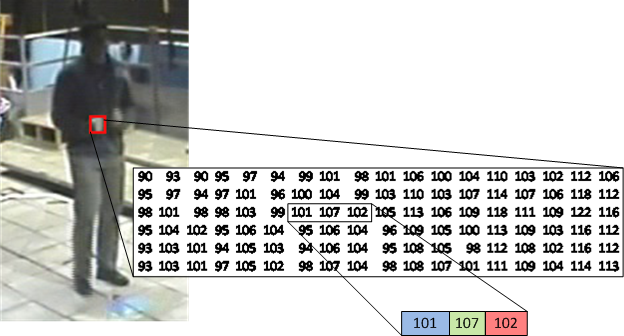
\includegraphics[scale=0.6]{img/ch5/opencv_mat}
\caption[Estructura de datos \textit{OpenCV Mat} ]{La estructura de datos \textit{OpenCV Mat} es un arreglo dividido en dos partes. Un encabezado, con información de tamaño, método utilizado para almacenar, dirección de localización de memoria de los datos. Un puntero a la zona de memoria donde se localiza la matriz de pixeles; números almacenados en forma contigua en el orden \textit{blue, green, red}, en el caso del espacio de colores RGB.}
\label{fig:mat}
\end{figure}

La zona es una matriz de números manejada por una estructura \textit{Mat}, en el caso de una imagen definida en el espacio RGB, se almacenan los valores de cada píxel, en forma contigua, en el orden: blue, green, y red.


\subsection{Biblioteca Boost}
Boost \cite{boost} se ha usado principalmente para evitar el problema que se encuentra al manipular archivos, operar con \textit{strings} de caracteres en C++. \textit{Boost} tiene varias bibliotecas utilitarias, y en este proyecto se han usado las que permiten manejar expresiones regulares, búsqueda de caracteres en una linea de \textit{strings}, reemplazo de caracteres, manipulación de archivos.(\textit{boost\:\:filesystem, boost\:\:system, boost\:\:program\_options, boost\:\:reg\_exp}).



\section{Descripción de Implementación}

Se elige \textit{C++} como lenguaje de programación para la implementación del sistema de software, y lenguaje de programación en \textit{Python} para el desarrollo de \textit{Scripts} que manipulan los datos de resultado y gráficas de desempeño. Los criterios de selección empleados para estos lenguajes de programación se listan a continuación.
 
\begin{itemize}
\item \textit{OpenCV} está optimizado para trabajar en \textit{C++}
\item \textit{C++} es un lenguaje de programación con orientación objetos. Se elige programación orientada a objetos por las características de \textit{encapsulación} y \textit{polimorfismo} que ofrece este tipo de programación. Estas características son aprovechadas por las clases que implementan el sistema para  encapsular los diferentes algoritmos que se desea verificar.
\item Los gráficos de desempeño fueron realizados en \textit{Matplotlib}\cite{matplotlib}, una biblioteca basada en \textit{Python} para construir gráficos. 
\item Experiencia de programación en ambos lenguajes
\end{itemize}

%La parte principal de la herramienta de software está constituida por los dos módulos localizados en la capa media, según la figura \ref{fig:arq_software}. , está compuesto por dos módulos principales e independientes. El módulo de \textit{Sistema Base} que permite incorporar y verificar los diferentes algoritmos, y el módulo que incluye diferentes métricas de evaluación de desempeño. Como señala el diagrama de componentes (operación), la figura \ref{fig:bgs_tasks}, los módulos son independientes y funcionan en tiempos diferentes. La salida del primero, es la entrada del segundo.
%
% \begin{figure}[h!]
%\centering
%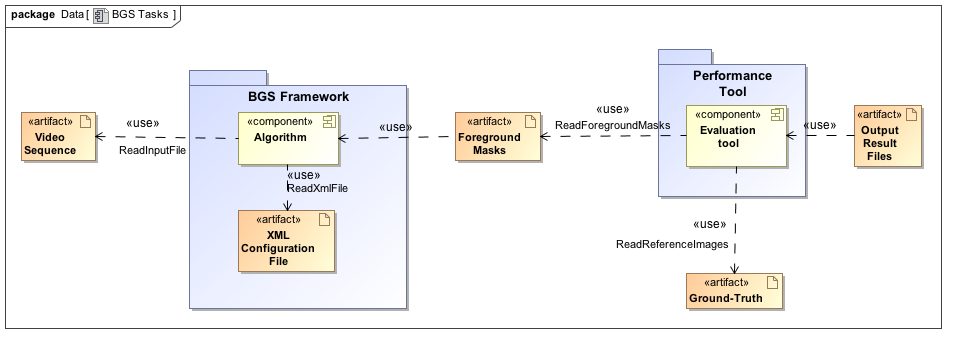
\includegraphics[scale=0.5]{img/ch5/BGS_Tasks}
%\caption[Diagrama de componentes]{Diagrama de operación de los componentes de software.}
%\label{fig:bgs_tasks}
%\end{figure}


\subsection{Sistema Base Integración Algoritmos de Visión por Computador}

%La entrada del \textit{Sistema} puede ser un archivo de video o  conjunto de imágenes secuenciales en cualquier formato (jpg, png, etc), y la salida son mascaras de siluetas (\textit{foreground}), generadas por el algoritmo seleccionado. Los resultados (mascaras) son almacenados en directorios independientes, (se crea un directorio por algoritmo configurado). De esta manera, se podrían ejecutar uno o más algoritmos en forma simultánea, dependiendo de un archivo \textit{xml} general de configuración. La configuración de cada uno de los algoritmos incluidos, también se realiza a través de archivos XML de configuración. Por cada algoritmo incluido en este \textit{framework} existe un archivo XML de configuración. Los archivos XML contienen parámetros necesarios que necesita el algoritmo para ser ajustado a los requerimientos de operación, entre estos se encuentran por ejemplo, la tasa de aprendizaje, valores por defecto de las distribuciones que modelan el fondo de imagen. 


%\subsection{Diagrama de clases}
%Se utilizó un patrón de diseño\cite{gamma_design_1995} \textbf{estrategia} (\textit{Strategy}) para implementar el \textit{Sistema Base}.  Los patrones de diseño\cite{gamma_design_1995} son esencialmente un conjunto de soluciones a problemas repetitivos que se encuentran en el desarrollo de software. Se aprovecha la experiencia de enfrentar un problema conocido, desde ese perspectiva   Utilizar un patrón de diseño es aprovechar la experiencia para enfrentar un problema conocido, re-usando una solución ya comprobada. Desde la perspectivaExisten otros patrones que podrían haber dado solución al problema de implementación de este sistema, se escogió  

Para abordar la implementación del sistema base, asimismo la herramienta de medición de métricas, se escogió el concepto de \textit{Diseño de Patrones}\cite{gamma_design_1995} como estructura base de las clases que implementan ambas soluciones. Diseño de Patrones (\textit{Design Patterns}\cite{gamma_design_1995}) es un conjunto de soluciones orientada a objetos de problemas repetitivos, que aprovechan la experiencia para enfrentar un problema conocido, re-usando una solución comprobada. En la literatura se los encuentra dividido en tres grupos, dependiendo de la relación entre clases y objetos que se usa. 

%Se escogió \textit{Diseño de Patrones}\cite{gamma_design_1995} para enfrentar el problema de la implementación del \textit{Sistema Base}. Diseño de patrones es un conjunto de soluciones orientada a objetos de problemas repetitivos, se aprovecha la experiencia para enfrentar un problema conocido, re-usando una solución comprobada. El desafío en elegir diseño de patrones es localizar el \textit{Patron} que se ajuste al problema que se quiere solucionar. Existen tres tipos de \textit{Patrones}\cite{gamma_design_1995}

\begin{itemize}
\item \textbf{Patrones Estructurales} (Structural Patterns)\textbf{:} Son Patrones que se usan para formar grandes estructuras de objetos y clases. Facilitan el trabajo de modificar estructuras de jerarquías de clases y sus asociaciones. Este tipo de patrones usa herencia para hacer composición de interfaces o implementaciones. Por ejemplo una clase que mezcla dos clases (múltiple herencia) en una clase, ésta clase combina las propiedades de ambas clases padres en una nueva clase independiente. De esta forma, este tipo de Patrones describe formas de componer objetos para agregar nuevas funcionalidades.
 \item \textbf{Patrones Creacionales} (Creational Patterns)\textbf{:} Son Patrones que tienen el propósito de facilitar el trabajo de creación (\textit{instanciación}), inicialización y configuración de objetos y clases. Independizan a un sistema de lo forma como los objetos son creados, compuestos, y representados. Se les denomina de esta manera porque crean cosas, como clases, implementación de interfaces, atributos, etc.
 \item \textbf{Patrones Comportamiento} (Behavioral Patterns)\textbf{:} Son Patrones orientados a la interacción y comunicación entre objetos, utilizan herencia para distribuir el comportamiento entre clases. Se usan para trabajar con algoritmos y la comunicación entre clases. Por ejemplo, un algoritmo usado por una clase es sólo parámetro que puede ser ajustado en tiempo de ejecución.
\end{itemize}

El desafío en diseño de patrones es localizar el \textit{Patrón} que se ajuste al problema que se quiere solucionar. Para esta implementación se escoge la alternativa de los \textit{Patrones de Comportamiento}, interesa seleccionar el tipo de algoritmo (\textit{comportamiento}) antes de la ejecución del programa principal, del sistema de software.  Es tipo de patrones permite definir una clase interfaz para exponer sólo los métodos (funcionalidades) necesarios para el funcionamiento del sistema de software. Dentro de esta categoría se estudiaron dos tipos de patrones que podrían haber sido adecuados para la implementación: Método de Plantilla (\textit{Template Method}), y Estrategía \textit(Strategy), escogiendo este último como el más adecuado.

El patrón del método plantilla, define una clase base de algoritmo (\textit{template}) y a partir de esa base se pueden crear sub-clases (clases hijos) que deriven las características particulares (comportamiento) del algoritmo que se desea exponer. El patrón de estrategia define un conjunto encapsulados de algoritmos que pueden ser intercambiados de acuerdo con alguna configuración en tiempo de ejecución, es decir se definen algoritmos en clases independientes y se elige alguno de ellos (selección de comportamiento) dependiendo de la estrategia en tiempo de ejecución. Se escoge el patrón de estrategia por la característica de seleccionar en tiempo de ejecución alguno de los algoritmos incorporados dentro del sistema. En cambio el método plantilla se requiere seleccionar los algoritmos a utilizar en tiempo de compilación.

\begin{figure}[h!]
\centering %%%
\subfigure[Patrón de Plantilla]
{\label{fig:plot15-1_1}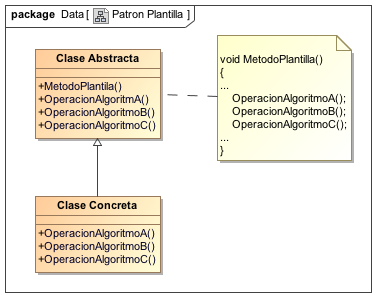
\includegraphics[width=80mm]{img/ch5/PatronPlantilla}}
\subfigure[Patrón Estrategia]
{\label{fig:plot15-2_1}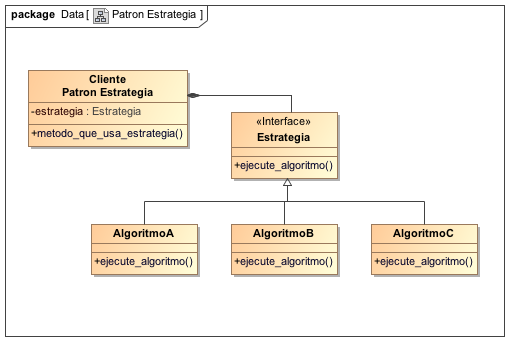
\includegraphics[width=80mm]{img/ch5/PatronEstrategia}}
\caption[Diagrama UML de patrones de diseño \textit{Plantilla} y \textit{Estrategia}]{Diagrama UML de los patrones estudiados para implementación del sistema base. El método plantilla  selecciona mediante sub-clases (herencia) en tiempo de compilación, el patrón de estrategia selecciona un algoritmo en tiempo de ejecución.}
\label{fig:ch5:patrones_de_diseno}
\end{figure}


\subsection{Diagrama de clases de implementación}



\begin{figure}[h!]
\centering
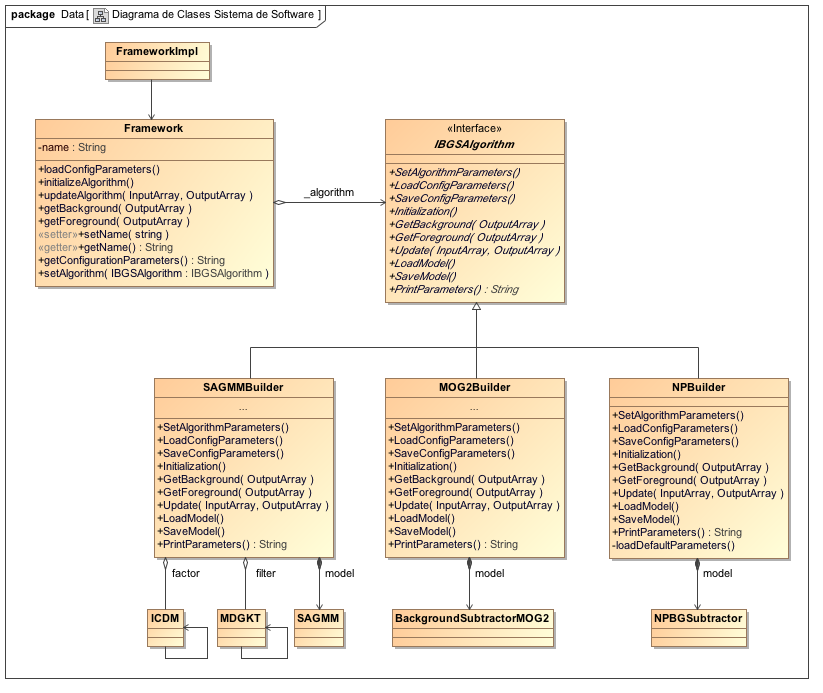
\includegraphics[scale=0.5]{img/ch5/BGSFramework}
\caption[Diagrama UML de clases del sistema base]{Diagrama UML de las distintas clases del sistema base. Se define una clase de tipo interfaz (\textit{IBSGAlgorithm}) que define y expone las principales funcionalidades de los algoritmos. Las clases \textit{<Algoritmo>}Builder se encargan de encapsular los algoritmos haciendo una composición de ellos. La clase \textit{Framework} implementa cada uno de los métodos de la clase \textit{IBSGAlgorithm} para que estos puedan ser usados por la implementación principal \textit{FrameworkImpl}.}
\label{fig:uml_framework}
\end{figure}

El patrón de diseño estrategia encapsula los algoritmos para hacerlos intercambiables, al ser invocados por algún cliente en tiempo de ejecución. Se basa en la idea de encapsular el comportamiento de la parte que cambia. Aprovecha la propiedad de ``\textit{polimorfismo}'' en programación orientada a objetos, para definir una interfaz común, sobre la cual los diferentes ``\textit{comportamientos}'' (algoritmos) son implementados. La figura \ref{fig:uml_framework} ilustra el diagrama de clases de la implementación para el sistema base.

\begin{itemize}
\item \textbf{Interfaz IBGSAlgorithm:} Es una clase abstracta de \textit{C++} que representa las funcionalidades principales de los algoritmos que se desean encapsular, para esto, se definen los principales métodos (funcionalidades) que la clase cliente debe llamar para usar un algoritmo.
\item \textbf{Clase \textit{<ALGORITMO>}Builder:} Es una clase concreta que integra un algoritmo en su definición, mediante \textit{composición} de un objeto algoritmo, esto significa que la clase \textit{Builder} es responsable de la creación y destrucción de las partes del objeto algoritmo. Esta clase hace una abstracción de cada algoritmo exponiendo únicamente las operaciones esenciales que se necesitan en la clase principal del sistema base. En la figura \ref{fig:uml_framework} se ilustran las clases \textit{\textbf{SAGMM}Builder}, \textit{\textbf{MOG2}Builder}, \textit{\textbf{NP}Builder}, las cuales corresponden a los algoritmos que se incluyen en el sistema base.
\item \textbf{Clase \textit{Framework}:} Es la clase principal que implementa cada uno de los métodos definidos en la clase interfaz \textit{IBGSFramework}.
\item \textbf{Programa Principal \textit{FrameworkImpl}:} Es la implementación del programa ejecutable, el cual crea las instancias de todos los algoritmos integrados en el sistema. Abajo se lista una parte de código ejemplo (Código \ref{FrameworkLabel}) que declara e inicializa los distintos objetos algoritmos, del tipo de clase \textit{Framework}.
\end{itemize}




\begin{lstlisting}[caption={Ejemplo de instanciación distintos objetos de algoritmos en programa principal. Cada algoritmo en este ejemplo, se declara como un tipo de la clase \textit{Framework} y luego se utilizan los métodos que configuran ese algoritmo.},label=FrameworkLabel]
{    ...
    Framework* mog2 = new Framework();
    mog2->setAlgorithm(new MOG2Builder());
    mog2->setName("MOG2");
    mog2->loadConfigParameters();
    mog2->initializeAlgorithm();

    Framework* np = new Framework();
    np->setAlgorithm(new NPBuilder(col,row,nch));
    np->setName("NP");
    np->loadConfigParameters();
    np->initializeAlgorithm();

    Framework *sagmm = new Framework();
    sagmm->setAlgorithm(new SAGMMBuilder());
    sagmm->setName("SAGMM");
    sagmm->loadConfigParameters();
    sagmm->initializeAlgorithm();
    ...
}
\end{lstlisting}

%se define una interfaz (clase abstracta en C++) para representar el comportamiento (\textit{IBGSFramework}) que se desea encapsular. Los distintos algoritmos son implementados como subclases de esta interfaz: \textit{SAGMMBuilder}, \textit{MOG2Builder}, \textit{NPBuilder}. Con este diseño, los algoritmos no están incluidos en la clase principal \textit{Framework}. Otros objetos podrían también hacer uso de \textit{IBGSFramework}, debido que no esta incorporada con la clase principal \textit{Framework}. Además, se pueden agregar más algoritmos (comportamientos) sin modificar las clases existentes o la clase principal.

%Las clases \textit{SAGMMBuilder}, \textit{MOG2Builder}, \textit{NPBuilder} (figura \ref{fig:uml_framework}) funcionan como clases especiales que crean las instancias de los algoritmos, hacen una abstracción de cada algoritmo exponiendo únicamente las operaciones esenciales que se necesitan en al framework.



El diagrama de secuencia en la figura \ref{fig:uml_sequence} es un ejemplo de los mensajes que son intercambiados entre un cliente (\textit{FramewrokImpl}), la clase \textit{Framework} y algún algoritmo definido en el sistema (\textit{SAGMM}, \textit{MOG2}, etc.). El cliente inicia enviando un mensaje al objeto \textit{Framework} para indicar el tipo de algoritmo a utilizar, método \textit{setAlgorithm}. Luego se realiza una configuración de parámetros del algoritmo que requiere para su funcionamiento (método \textit{LoadConfigParameters}). La configuración de un algoritmo se realiza por medio de un archivo XML, para esto se aprovecha una funcionalidad de \textit{OpenCV} para leer archivos de configuración en formato XML. El método \textit{initializeAlgorithm} se encarga de finalizar la configuración del algoritmo (con los parámetros leidos desde el archivo XML). Una vez que los pasos previos han finalizado, el cliente esta en condiciones de leer las imágenes (mascaras) que al algoritmo esta procesando.


\begin{figure}[h!]
\centering
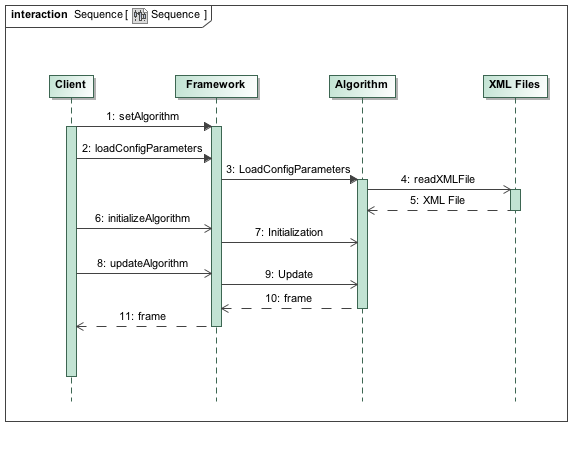
\includegraphics[scale=0.5]{img/ch5/Sequence}
\caption[Diagrama de secuencia]{Diagrama de secuencia de ejecución de un algoritmo}
\label{fig:uml_sequence}
\end{figure}


\subsection{Herramienta de evaluación de desempeño}
Se basa principalmente de una clase denominada ``\textit{Performance}'' (ver diagrama UML de figura \ref{fig:uml_evaluacion}), compuesta de una serie de operaciones (métodos) encargados de realizar los diferentes cómputos de desempeños. Se han dispuesto una serie de métodos públicos (\textit{getters}), que permiten acceder a un valor de atributo privado dentro de la clase, para obtener el valor de las distintas métricas. Asimismo, se han definido un grupo de estructuras que permite agrupar y almacenar las diferentes métricas por tipo de medida, en la medida que van realizando las comparaciones entre una imagen y su referencia. 

\begin{itemize}
\item \textbf{\textit{Similarity} Struct:} Contiene las métricas de similaridad: \textit{DScore}, \textit{MSSIM}, y relación señal a ruido \textit{PSNR}. Estás métricas son obtenidas a nivel \textit{frames}, es decir, la comparación se realiza entre dos imágenes.
\item \textbf{\textit{ContingencyMatrix} Struct:} Mantiene los datos resultante de la matriz de confusión. Son métricas obtenidas por comparación a nivel de pixel, de una imagen de entrada con su imagen de referencia.
\item \textbf{\textit{CommonMetrics} Struct:} Es una estructura que mantiene las métricas comunes, de \textit{sensitividad} y \textit{especificidad}. 
\item \textbf{\textit{StatMetrics} Struct:} Estructura compuesta que almacena los valores de media y mediana de las métricas comunes.
\item \textbf{\textit{GlobalMetrics} Struct:} es una estructura compuesta que almacena un sumario de todas las métricas.
\end{itemize}


\begin{figure}[h!]
\centering
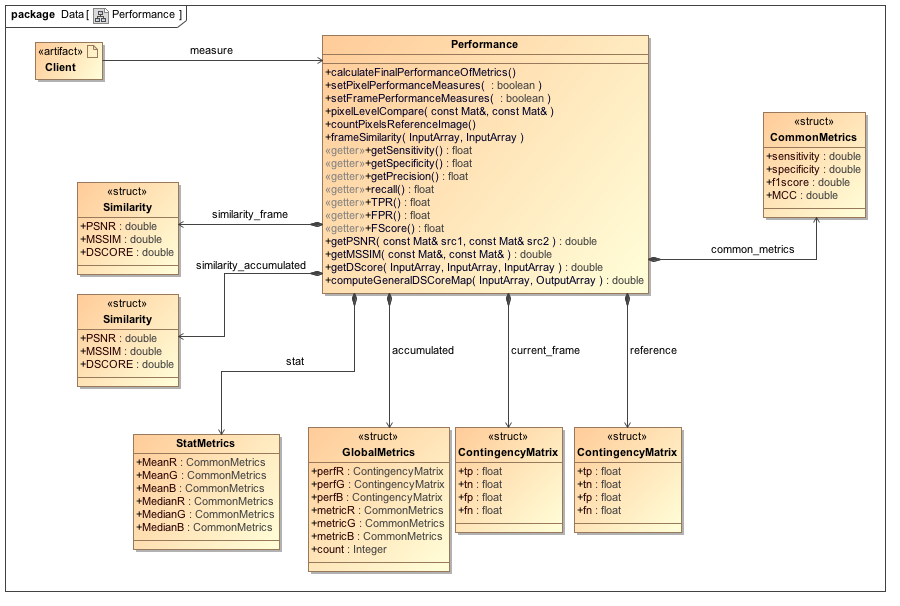
\includegraphics[scale=0.5]{img/ch5/Performance}
\caption[Diagrama UML herramienta de evaluación]{Diagrama UML herramienta de evaluación}
\label{fig:uml_evaluacion}
\end{figure}


\subsection{Operación de la implementación}
En la imagen de la figura \ref{fig:diagrama_bloques} se muestra un esquema de funcionamiento de la implementación de las clases del sistema base en dos programas ejecutables. De manera informativa se muestra ambos programas funcionando de manera combinada, pero el funcionamiento de ambos es totalmente independiente. El programa ejecutable \textit{bgs\_framework}, bloque localizado en la parte superior de la figura \ref{fig:diagrama_bloques}, es una implementación de la clase \textit{Framework}, el programa recibe de entrada un secuencia de imágenes desde el conjunto de datos MuHAVI, lee desde un archivo XML (localizado en un directorio local donde se ejecuta la aplicación) y genera un conjunto de imágenes resultantes (mascaras de siluetas) que van siendo almacenadas en un directorio local a medida que se ejecuta la aplicación.


En una segunda parte, los resultados son comparados con las imágenes de referencia (\textit{ground-truth}) que proporciona MuHAVI, mediante el programa \textit{pmbgs}. Esta aplicación es una implementación que contiene un objeto de la clase \textit{Performance}, es decir declara este objeto y luego lo define, y posteriormente utiliza los métodos que proporciona esta clase para ir leyendo las distintas métricas resultantes de la comparación que se está realizando.

\begin{figure}[h!]
\centering
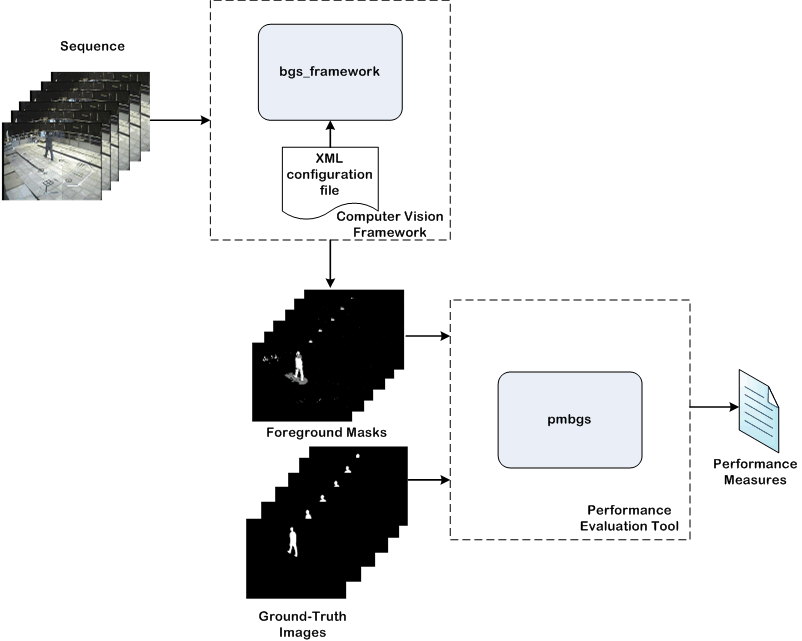
\includegraphics[scale=0.5]{img/ch5/block_diagram_application}
\caption[Diagrama en bloques de operación de ambos elementos, sistema base de algoritmos y herramienta de evaluación de desempeño]{Diagrama en bloques que señala la operación del sistema base de los algoritmos y la herramienta de evaluación de desempeño, sólo de manera informativa se muestran ambos módulos funcionando en forma combinada. El sistema base de algoritmos obtiene parámetros de configuración de un archivo XML y procesa una secuencia de imágenes (MuHAVI). La herramienta de evaluación, posteriormente \textit{off-line}) compara las imágenes resultantes del procesamiento del algoritmo con las imágenes de referencia (ground-truth) que proporciona MuHAVI, generando como resultado un archivo de texto con las métricas de desempeño por secuencia. }
\label{fig:diagrama_bloques}
\end{figure}

%que se hace una descripción además de los detalles de solución para finalizar con un producto de software que cumple con las ideas propuesta al comienzo del proyecto. llevar a cabo la implementación del software propuesto en los requerimientos.
\section{Resumen}
Este capítulo hace una descripción de las distintas actividades realizadas  en la implementación del sistema de software de este proyecto, así como también una descripción de las diferentes clases \textit{C++} desarrolladas, a nivel de diagrama UML, que conforman el sistema base de algoritmos y mediciones de desempeño del proyecto. Sin una idea previa, para utilizar alguna metodología conocida de desarrollo de software, todo el avance dentro del proyecto, las diferentes etapas que se fueron ejecutando y finalizando dan cuenta de una metodología muy parecida (sino igual) a un modelo del tipo \textit{Waterfall}. Todas las actividades siguieron una linea secuencial, que se inició con la captura de los requerimientos, luego continuó con el diseño de la solución, posteriormente la implementación, para finalizar con la puesta en marcha, verificación y mantenimiento (solución de problemas encontrados). Afortunadamente, desde el punto de vista de esta metodología, los requerimientos fueron constante y no hubo variación de ellos durante el transcurso del proyecto. Uno de los problemas críticos dentro de esta metodología, consiste exactamente en el cambio de los requerimientos, cualquier modificación de estos, requiere una nueva revisión desde el comienzo, lo que en definitiva significa alargar los plazos del proyecto. La lógica de secuencia de las secciones dentro de este capítulo describen en cierta forma el proceso de desarrollo seguido en la etapa de implementación. 

Con respecto a las diferentes decisiones de implementación, muchas de ellas fueron tomadas basadas en experiencias anteriores, que ayudarían a rebajar los tiempos de implementación. Ese es el caso por ejemplo, de utilizar lenguaje de programación C++ y no otro similar como \textit{Java}, también por compatibilidad con la plataforma de visión por computador \textit{OpenCV}, el cual en su mayor parte esta desarrollado en \textit{C++}, pero es compatible con otros lenguajes de programación. Con respecto a la utilización de patrones de diseño, esta decisión sigue la lógica de reutilizar código y experiencias documentadas, además de asegurar un código más robusto (problemas de punteros, asignación de memoria, \textit{bugs}). Sin embargo, utilizar patrones requirió tiempo para escoger el más adecuado, mismo tiempo que a lo mejor se podría haber utilizado para desarrollar desde cero. En síntesis, siempre queda una incertidumbre cuál alternativa escoger. 

Finalmente el sistema de software fue implementado y verificado con extensas pruebas sobre el conjunto de datos MuHAVI, el siguiente capítulo se dedica exclusivamente a revisar los resultados de las métricas de evaluación obtenidas con la herramienta de evaluación implementada al ser utilizada con las imágenes resultantes del sistema de algoritmos.

 